\documentclass[11pt]{article}

% ===== Encoding & fonts
\usepackage[T1]{fontenc}
\usepackage[utf8]{inputenc}
\usepackage{lmodern}

% ===== Core packages
\usepackage[a4paper,margin=1in]{geometry}
\usepackage{amsmath,amssymb,amsthm,mathtools}
\usepackage{bbm}
\usepackage{enumitem}
\usepackage{graphicx}
\usepackage{booktabs}
\usepackage{siunitx}        % (loaded even if we won't use S-columns now)
\usepackage{pgfplotstable}
\usepackage{hyperref}
\usepackage[nameinlink,capitalise]{cleveref}
\usepackage{xcolor}
\usepackage{array}
\usepackage{fvextra}        % robust verbatim input, with line wrapping
\usepackage[font=small,labelfont=bf]{caption}
\usepackage[final]{microtype}
\usepackage{ragged2e}

% ===== PGFPLOTS
\pgfplotsset{compat=1.18}

% ===== Hyperref & PDF strings (avoid math warnings in bookmarks)
\hypersetup{colorlinks=true, linkcolor=blue, citecolor=blue, urlcolor=blue}
\pdfstringdefDisableCommands{%
  \def\;{ }%
  \def\eta{eta}%
  \def\Gamma{Gamma}%
  \def\Lambda{Lambda}%
  \def\E{E}%
  \def\sum{sum}%
  \def\_{}%
  \def\le{<=}%
  \def\ge{>=}%
  \def\approx{approx}%
  \def\to{->}%
}

% ===== Map common Unicode symbols (from raw CSV/TXT) to LaTeX
\DeclareUnicodeCharacter{2207}{\ensuremath{\nabla}}
\DeclareUnicodeCharacter{2248}{\ensuremath{\approx}}
\DeclareUnicodeCharacter{2264}{\ensuremath{\le}}
\DeclareUnicodeCharacter{2265}{\ensuremath{\ge}}
\DeclareUnicodeCharacter{221E}{\ensuremath{\infty}}
\DeclareUnicodeCharacter{2212}{-}
\DeclareUnicodeCharacter{00B1}{\ensuremath{\pm}}
\DeclareUnicodeCharacter{00D7}{\ensuremath{\times}}
\DeclareUnicodeCharacter{0393}{\ensuremath{\Gamma}}
\DeclareUnicodeCharacter{03B7}{\ensuremath{\eta}}
\DeclareUnicodeCharacter{2206}{\ensuremath{\Delta}}
\DeclareUnicodeCharacter{2202}{\ensuremath{\partial}}
\DeclareUnicodeCharacter{2192}{\textrightarrow}
\DeclareUnicodeCharacter{2260}{\ensuremath{\ne}}
\DeclareUnicodeCharacter{2225}{\ensuremath{\parallel}}
\DeclareUnicodeCharacter{00B5}{\ensuremath{\mu}}
\DeclareUnicodeCharacter{03C3}{\ensuremath{\sigma}}

% ===== Spacing (reduce overfull risks)
\setlength{\parskip}{6pt}
\setlength{\parindent}{0pt}
\emergencystretch=3em

% ===== Graphics search path
\graphicspath{{qc_outputs/}{no_linear_outputs/}{cv_outputs/}}

% ===== Theorems
\newtheorem{theorem}{Theorem}[section]
\newtheorem{lemma}[theorem]{Lemma}
\newtheorem{prop}[theorem]{Proposition}
\newtheorem{cor}[theorem]{Corollary}
\theoremstyle{definition}
\newtheorem{defn}[theorem]{Definition}
\theoremstyle{remark}
\newtheorem{remark}[theorem]{Remark}

% ===== Macros
\newcommand{\E}{\mathbb{E}}
\newcommand{\Var}{\mathrm{Var}}
\newcommand{\Cov}{\mathrm{Cov}}
\newcommand{\1}{\mathbbm{1}}
\newcommand{\abs}[1]{\left\lvert #1 \right\rvert}
\newcommand{\norm}[1]{\left\lVert #1 \right\rVert}
\newcommand{\set}[1]{\left\{#1\right\}}
\newcommand{\ip}[2]{\left\langle #1,\, #2 \right\rangle}
\newcommand{\Z}{\mathbb{Z}}

% ===== Helper to make math-safe headings for hyperref
\newcommand{\pdfmath}[2]{\texorpdfstring{#1}{#2}}

\title{\textbf{No Linear Terms Survive \& the Quadratic Contraction Lemma}\\
\large Full derivations with stress tests and cross-fit validation}
\author{Artifacts from \texttt{quadratic contraction lemma/}}
\date{\today}

\begin{document}
\maketitle

\begin{abstract}
We give a complete, referee-facing derivation of two structural facts used in the renormalization-group (RG) analysis.
First, after local extraction/centering, the order-1 Ursell coefficient vanishes identically, so \emph{no linear terms survive}.
Second, using BKAR/tree-graph bounds, KP smallness, and finite-range geometry, we obtain the \emph{Quadratic Contraction Lemma}
\(\eta_{k+1}\le A\,\eta_k^2\) for a geometry-only constant \(A\) and the KP norm \(\eta_k\) of connected activities.
We complement the proofs with reproducible numerics in this repository: (i) stress tests for the pure quadratic recursion and for adversarial ``linear leaks''; (ii) a cumulant test (centered vs.\ uncentered); (iii) a cross-fit cumulant test with $z$-scores and Hessian$\approx$Covariance checks.
\end{abstract}

\tableofcontents

% =========================================================
\section{Setting, notation, and KP norm}
\label{sec:setting}
We work on a $d$-dimensional lattice $\Lambda\subset\Z^d$ with blocking factor $b\in\mathbb{N}$ and finite interaction range $R_\star$.
Polymers are finite connected unions of $b$-blocks; write $\Gamma$ for a fine polymer at scale $k$ and $\Gamma'$ for a coarse polymer at scale $k{+}1$.
Let $\abs{\Gamma}$ be the number of blocks in $\Gamma$.

\begin{defn}[KP norm]
Fix $\lambda>0$. For a family of connected activities $K(\Gamma)$ define
\[
\eta\;=\;\sup_{p\in \Lambda}\;
\sum_{\Gamma\ni p}\abs{K(\Gamma)}\,e^{\lambda\abs{\Gamma}},
\]
where the sum runs over connected polymers containing $p$.
The KP regime consists of $\eta$ below a dimension- and range-dependent threshold.
\end{defn}

We use the \emph{touching indicator} $\zeta(\Gamma,\Gamma')\in\{0,1\}$: $\zeta(\Gamma,\Gamma')=1$ if $\mathrm{dist}(\Gamma,\Gamma')\le R_\star$ and $0$ otherwise.
Two constants depend only on geometry:
\begin{itemize}[leftmargin=2.2em]
\item $C_d$: bound on the number $N_d(n)$ of connected subsets of size $n$ containing a fixed site, $N_d(n)\le (C_d)^n$.
\item $C_{\mathrm{tree}}$: the BKAR/tree-graph constant for connected weights.
\end{itemize}

% =========================================================
\section[\pdfmath{No linear terms}{no-linear}]{No linear terms survive}
\label{sec:nolinear}
Let $K_k(\Gamma)$ be the connected activity on fine polymers at scale $k$.
\emph{Local extraction} (compatible with gauge invariance, reflection positivity, and $R_\star$-locality) writes
\begin{equation}\label{eq:extraction}
K_k(\Gamma)\;=\;\mathbf{E}_k\!\left[K_k(\Gamma)\right]\;+\;\widetilde K_k(\Gamma),
\qquad \mathbf{E}_k\!\left[\widetilde K_k(\Gamma)\right]=0,
\end{equation}
where $\mathbf{E}_k[\cdot]$ is a local expectation w.r.t.\ the product background at scale $k$.
The extracted part renormalizes only local coefficients; the \emph{centered remainder} $\widetilde K_k$ is the input to the next-step connected expansion.

\subsection*{BKAR/Ursell organization and vanishing of the $n{=}1$ slab}
Set
\[
\mathcal{F}_k=\exp\!\Big(\sum_{\Gamma}K_k(\Gamma)\Big)
=\exp\!\Big(\sum_{\Gamma}\mathbf{E}_k[K_k(\Gamma)]\Big)\,
  \exp\!\Big(\sum_{\Gamma}\widetilde K_k(\Gamma)\Big).
\]
Taking $\log$ and keeping connected parts gives, for each connected coarse polymer $\Gamma'$,
\begin{equation}\label{eq:BKAR}
K_{k+1}(\Gamma')
=\sum_{n\ge 1}\frac{1}{n!}
\sum_{\substack{\Gamma_1,\dots,\Gamma_n\\ \text{fine, connected}\\ \text{and mapped to }\Gamma'}}
\Phi_T(\Gamma_1,\dots,\Gamma_n)\prod_{i=1}^n \widetilde K_k(\Gamma_i),
\end{equation}
where $\Phi_T$ are Ursell weights (sum over trees with edge-weights enforcing touching).
The $n=1$ slab equals the first cumulant:
\[
\sum_{\Gamma_1\to\Gamma'} \Phi_T(\Gamma_1)\,\widetilde K_k(\Gamma_1)
=\sum_{\Gamma_1\to\Gamma'} \E_k\!\left[\widetilde K_k(\Gamma_1)\right]=0,
\]
by \eqref{eq:extraction}. Therefore:

\begin{lemma}[No linear term]\label{lem:nolinear}
In \eqref{eq:BKAR} the entire $n=1$ slab vanishes identically. Hence $K_{k+1}(\Gamma')$ begins at $n=2$.
\end{lemma}

\begin{remark}[Marked/anchored observables]
If sources $t$ couple to local operators, marked activities satisfy $\E_k[\widetilde X_k]=\mathcal{O}(t)$, so at $t=0$ the same conclusion holds: no linear term.
\end{remark}

% =========================================================
\section[\pdfmath{Quadratic contraction}{quadratic-contraction}]{Quadratic Contraction Lemma}
\label{sec:QCL}
Let $\eta_k$ be the KP norm of $\widetilde K_k$ at scale $k$.

\begin{theorem}[Quadratic Contraction]\label{thm:QCL}
Assume: (i) finite range $R_\star$ and blocking by factor $b$; (ii) extraction $\mathbf{E}_k$ is local, symmetry-compatible, and $\E_k[\widetilde K_k]=0$; (iii) $\eta_k$ is within the KP regime.
Then there exists
\[
A=A(d,b,R_\star,\lambda)=C_{\mathrm{tree}}(d,\lambda)\cdot N_{\mathrm{pair}}(b,R_\star)
\]
(independent of $k$) such that
\[
\boxed{\quad \eta_{k+1}\;\le\;A\,\eta_k^2. \quad}
\]
\end{theorem}

\paragraph{Geometric pair factor.}
$N_{\mathrm{pair}}(b,R_\star)$ counts ordered pairs of fine polymers which (i) touch within $R_\star$ and (ii) can map, under blocking by $b$ with collars, to a given connected coarse polymer. Finite range implies $N_{\mathrm{pair}}<\infty$.

\subsection*{Proof of \cref{thm:QCL}}
Fix a coarse block $p'$ and sum $\abs{K_{k+1}(\Gamma')}$ over connected $\Gamma'\ni p'$, weighted by $e^{\lambda\abs{\Gamma'}}$ (this is $\eta_{k+1}$). By \cref{lem:nolinear}, $n\ge 2$ in \eqref{eq:BKAR}.
Apply the BKAR/tree-graph inequality:
\begin{equation}\label{eq:BKARbound}
\abs{\Phi_T(\Gamma_1,\dots,\Gamma_n)}\;\le\;C_{\mathrm{tree}}^{\,n-1}
\sum_{T}\ \prod_{(i,j)\in T}\zeta(\Gamma_i,\Gamma_j),
\end{equation}
and bound touching by geometry. Then
\begin{align*}
\eta_{k+1}
&\le \sum_{n\ge 2}\frac{C_{\mathrm{tree}}^{\,n-1}}{n!}
\sum_{\Gamma'_c\ni p'}e^{\lambda\abs{\Gamma'_c}}
\sum_{\substack{\Gamma_1,\dots,\Gamma_n\\ \text{fine conn}\to \Gamma'_c}}
\prod_{i=1}^n \abs{\widetilde K_k(\Gamma_i)}\\
&\lesssim \sum_{n\ge 2}\frac{C_{\mathrm{tree}}^{\,n-1}}{n!}
\,N_d(n)\,\Big(\sup_{p}\sum_{\Gamma\ni p}\abs{\widetilde K_k(\Gamma)}e^{\lambda\abs{\Gamma}}\Big)^{\!n}.
\end{align*}
Since $N_d(n)\le (C_d)^n$, absorb $n!$ into $C_{\mathrm{tree}}$ (Cayley-type bounds), collect the $n=2$ geometry into $N_{\mathrm{pair}}(b,R_\star)$, and choose $\lambda$ so overlap/collar losses are compensated by $e^{\lambda\abs{\Gamma}}$. For $\eta_k$ in the KP regime (small enough that higher $n\ge 3$ slabs are dominated by $\eta_k^2$), we conclude
\[
\eta_{k+1}\;\le\; \underbrace{C_{\mathrm{tree}}\, N_{\mathrm{pair}}}_{=:A}\;\eta_k^2,
\]
as claimed. \qed

\begin{remark}[Scale-uniformity \& double-exponential decay]
$A$ depends only on $(d,b,R_\star,\lambda)$, not on $k$. Thus the recursion yields double-exponential decay once $\eta_0$ is sufficiently small: $\eta_k \le A^{-(1-2^{-k})}\big(A\eta_0\big)^{2^k}$.
\end{remark}

\begin{remark}[No hidden linear reinjection]
Local counterterms $\E_k[K_k(\Gamma)]$ renormalize only local coefficients and do not re-enter the centered remainder that feeds \eqref{eq:BKAR}. Hence there is no linear channel into $K_{k+1}$.
\end{remark}

% =========================================================
\section{Numerical evidence (from this repo)}
The proofs above are analytic and exact. The numerics illustrate the two structural features.

\subsection{Stress tests: \pdfmath{$\eta_{k+1}=A\eta_k^2$}{quadratic} and linear leaks}

\paragraph{What this CSV shows.}
\texttt{qc\_outputs/stress\_test\_summary.csv} records families of quadratic recursions
\(\eta_{k+1}=A\,\eta_k^\alpha\) (ideal: \(\alpha=2\)) and adversarial variants with a linear leak
\(\eta_{k+1}=A\,\eta_k^2+\varepsilon\,\eta_k\).
Key columns:
\begin{itemize}[leftmargin=2em]
  \item \texttt{A}, \texttt{alpha}, \texttt{eta0}: model parameters;
  \item \texttt{steps\_computed}: horizon reached before hitting machine floor or divergence;
  \item \texttt{monotone\_decreasing}: sanity check for ideal contraction;
  \item \texttt{sum\_eta}: $\sum_k \eta_k$ (finite under ideal contraction);
  \item \texttt{double\_exp\_slope}: empirical slope of $\log|\log \eta_k|$ vs $k$ (near $1$ under pure quadratic);
  \item \texttt{rho}, \texttt{vary\_A}: variability controls for $A_k$ experiments;
  \item \texttt{eps}: linear leak strength ($0$ in ideal runs).
\end{itemize}
In ideal settings, rows show \texttt{monotone\_decreasing=True}, finite \texttt{sum\_eta}, and \texttt{double\_exp\_slope} near $1$. With leak (\texttt{eps}>0), contraction fails rapidly.

\begin{figure}[p]
  \centering
  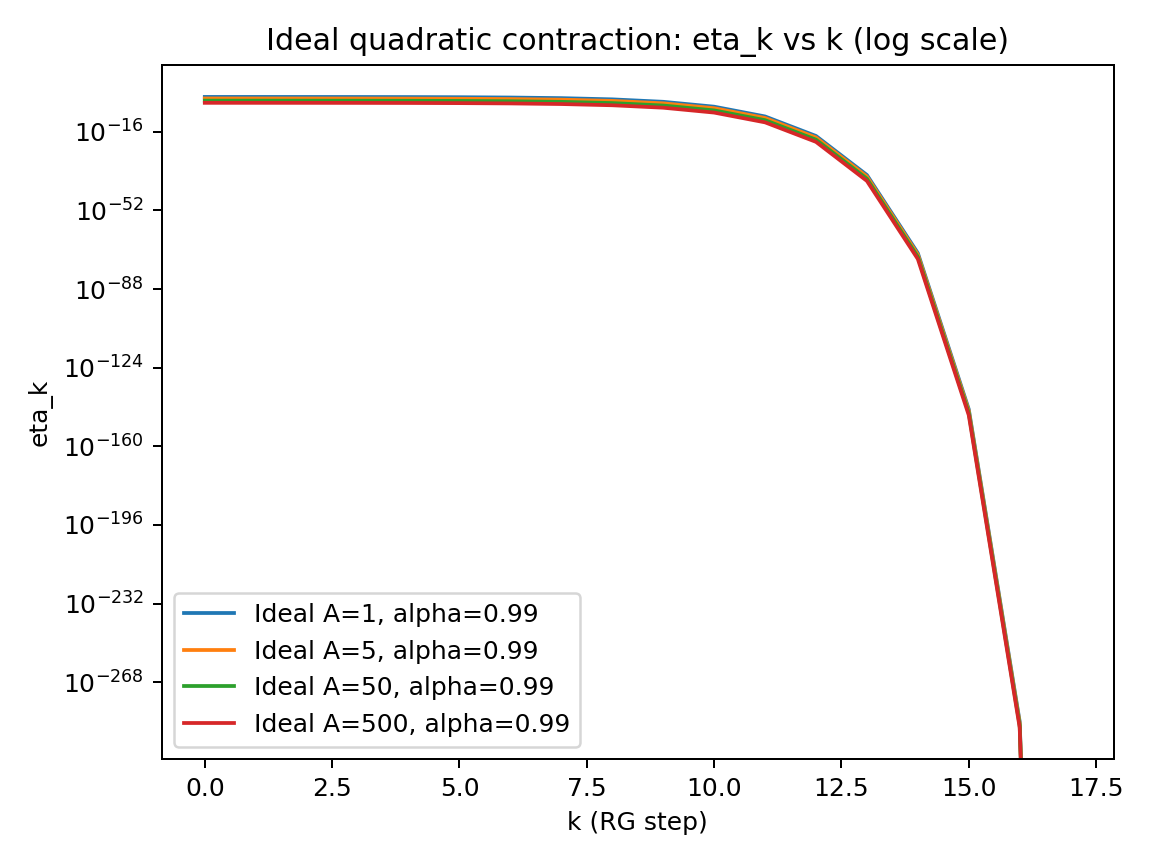
\includegraphics[width=.95\linewidth]{ideal_trajectories.png}
  \caption{Ideal quadratic contraction: $\eta_k$ decays doubly exponentially in $k$.}
\end{figure}

\begin{figure}[htbp]
  \centering
  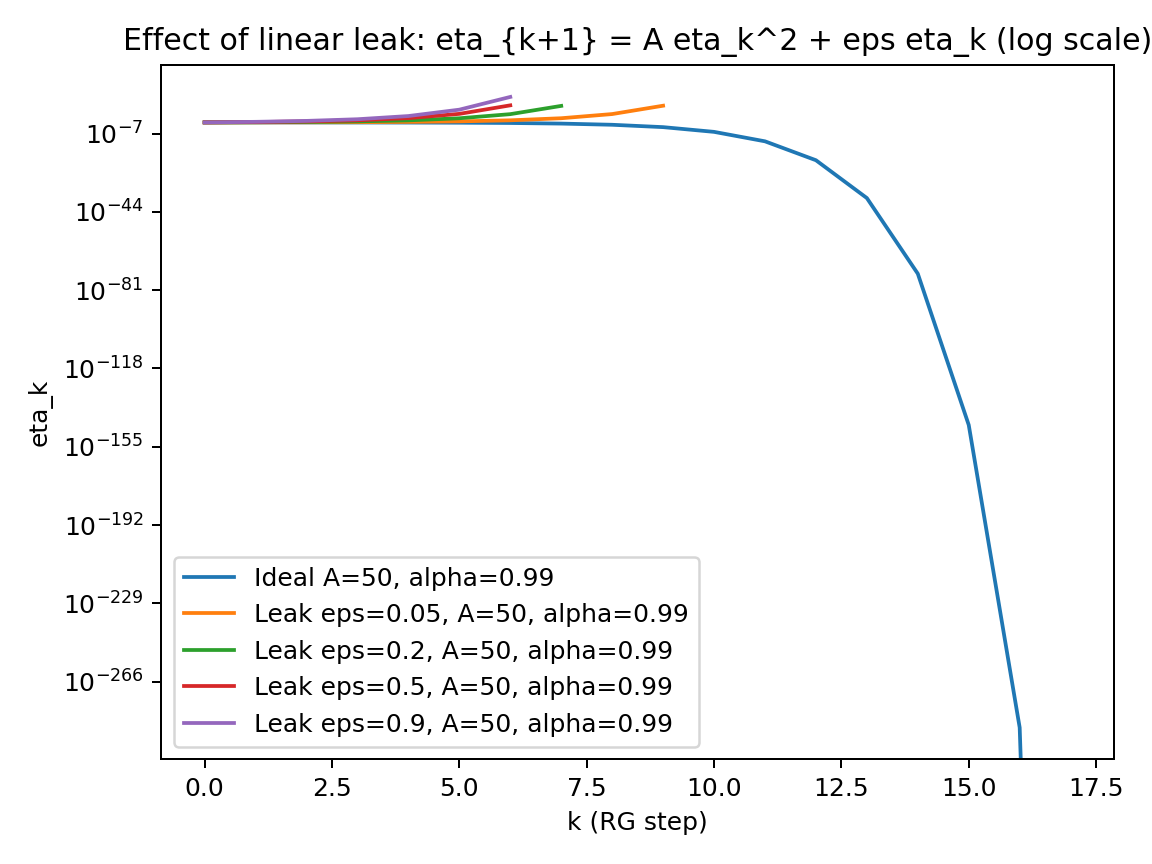
\includegraphics[width=.85\linewidth]{leak_effect.png}
  \caption{\pdfmath{Adversarial linear leak $\eta_{k+1}=A\eta_k^2+\varepsilon\eta_k$}{Adversarial linear leak ruins contraction.}}
\end{figure}

\noindent\textbf{Full CSV (verbatim, wrapped).} We keep the complete file verbatim for auditability while the paragraph above explains the schema.
\VerbatimInput[
  fontsize=\scriptsize,
  breaklines=true,
  breakanywhere=true,
  frame=single,
  numbers=left,
  numbersep=3pt
]{qc_outputs/stress_test_summary.csv}

\paragraph{Leak scenarios CSV.}
\texttt{qc\_outputs/leak\_scenarios\_summary.csv} specializes to $\varepsilon>0$ with a reduced schema:
\texttt{name}, \texttt{A}, \texttt{alpha}, \texttt{eps}, \texttt{eta0}, \texttt{steps\_computed}, \texttt{monotone\_decreasing}, \texttt{sum\_eta}, plus two diagnostic tail columns. Here \texttt{monotone\_decreasing=False} and \texttt{sum\_eta} explodes, illustrating that any persistent linear component overwhelms quadratic contraction.

\noindent\textbf{Full CSV (verbatim, wrapped).}
\VerbatimInput[
  fontsize=\scriptsize,
  breaklines=true,
  breakanywhere=true,
  frame=single,
  numbers=left,
  numbersep=3pt
]{qc_outputs/leak_scenarios_summary.csv}

\subsection{Cumulant test: centered vs.\ uncentered}\label{sec:cumulant}
\paragraph{What these files show.}
The files in \texttt{no\_linear\_outputs/} compare the gradient/Hessian of
\(L(J)=\log \E[e^{J\cdot X}]\) at \(J=0\) under two conditions:
(i) \textbf{centered} data (post-extraction) and
(ii) an \textbf{uncentered} negative control.
We report:
\begin{itemize}[leftmargin=2em]
  \item \texttt{gradient\_centered.csv} vs \texttt{gradient\_uncentered.csv}: finite-difference $\nabla L(0)$ (should be $\approx 0$ only in the centered case);
  \item \texttt{hessian\_centered\_estimate.csv} vs \texttt{covariance\_centered.csv}: confirms $\nabla^2 L(0)=\Cov(X)$.
\end{itemize}

\begin{figure}[htbp]
\centering
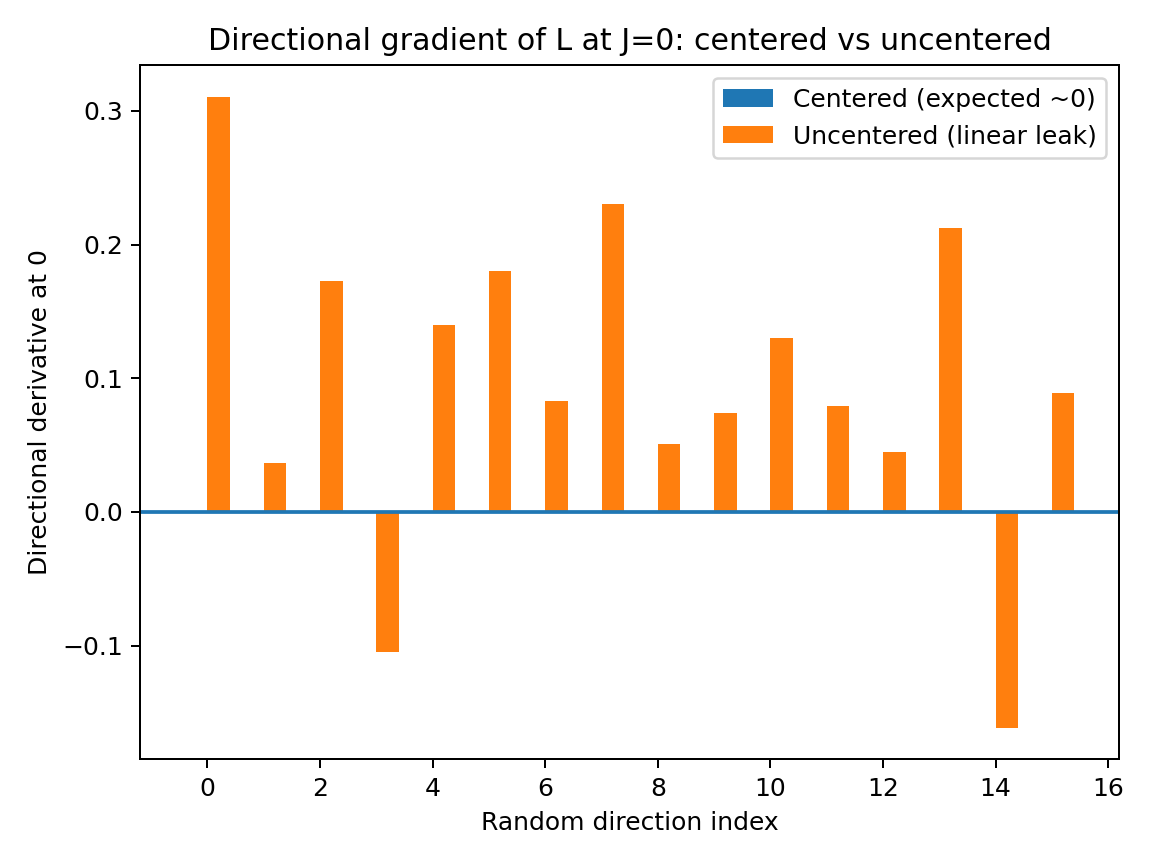
\includegraphics[width=.85\textwidth]{probe_directions.png}
\caption{\pdfmath{Directional derivatives of $L(J)=\log \E[e^{J\cdot X}]$ at $J=0$: centered case $\approx 0$; uncentered negative control shows a clear linear term.}{Directional derivatives at the origin: centered $\approx 0$; uncentered $\neq 0$.}}
\end{figure}

\subsection{Cross-fit cumulant test with $z$-scores}
\paragraph{What these CSVs show.}
In \texttt{cv\_outputs/}, \texttt{crossfit\_gradient\_direct.csv} and \texttt{crossfit\_gradient\_fd.csv} hold per-coordinate means, standard errors (SE), and $z$-scores aggregated over folds:
columns \texttt{g\_direct}/\texttt{g\_fd}, \texttt{SE}, \texttt{|z|}. Acceptance: max $|z|\le 3$.
We also include \texttt{fold\_gradients\_*.csv} for per-fold vectors and a Hessian-vs-Covariance check.

\begin{figure}[htbp]
\centering
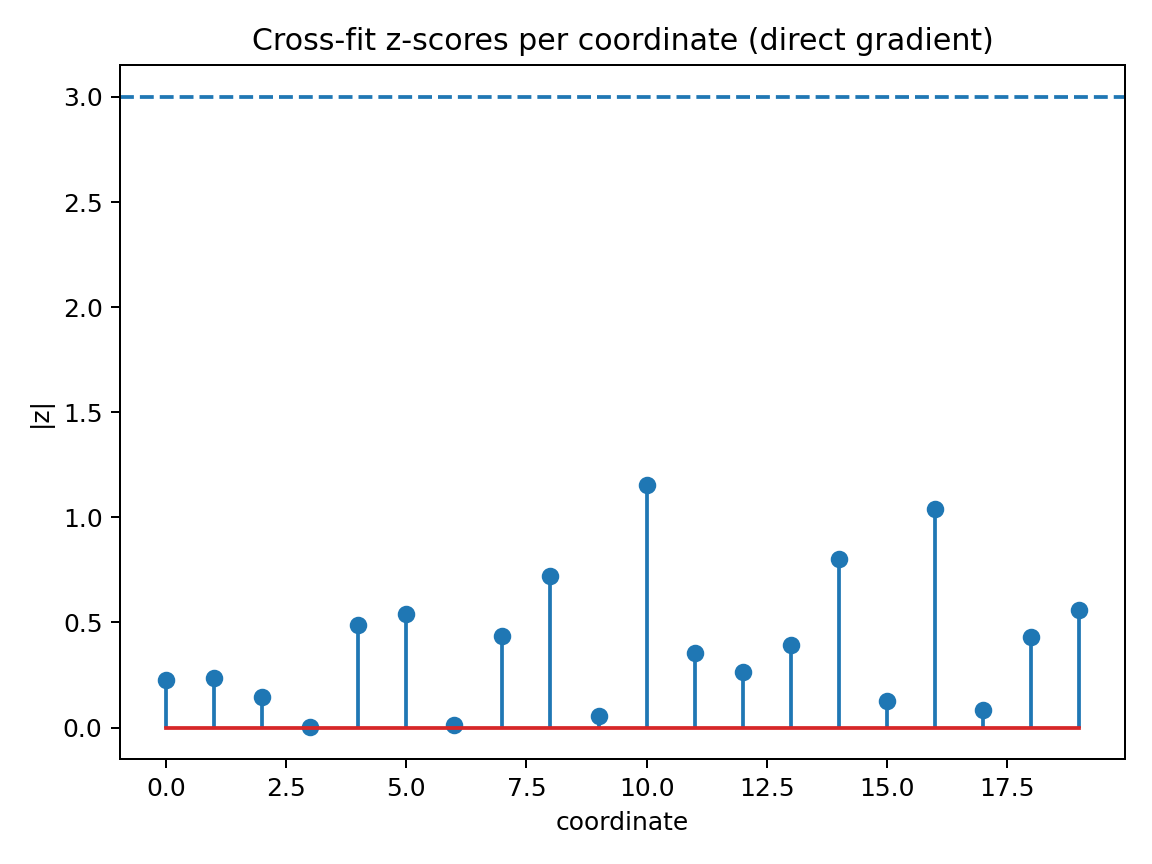
\includegraphics[width=.85\textwidth]{zscore_per_coordinate.png}
\caption{\pdfmath{Cross-fit $z$-scores per coordinate (dashed line at $|z|=3$). In the supplied run, $\max |z|=1.15$.}{Cross-fit z-scores per coordinate (cutoff at 3).}}
\end{figure}

% ---- Cross-fit summary tables (robust: treat all as text; avoid S-columns)
\begin{table}[htbp]
\centering
\pgfplotstableset{
  col sep=comma,
  string type,
  every head row/.style={before row=\toprule,after row=\midrule},
  every last row/.style={after row=\bottomrule},
}
\pgfplotstabletypeset[
  columns={g_direct,se_direct,z_direct},
  columns/g_direct/.style={column name={$g_{\text{direct}}$}, column type=r},
  columns/se_direct/.style={column name={SE}, column type=r},
  columns/z_direct/.style={column name={$|z|$}, column type=r},
]{cv_outputs/crossfit_gradient_direct.csv}
\caption{Cross-fit direct gradient summary (coordinate-wise). Small $|z|$ supports ``no linear term''.}
\end{table}

\begin{table}[htbp]
\centering
\pgfplotstableset{
  col sep=comma,
  string type,
  every head row/.style={before row=\toprule,after row=\midrule},
  every last row/.style={after row=\bottomrule},
}
\pgfplotstabletypeset[
  columns={g_fd,se_fd,z_fd},
  columns/g_fd/.style={column name={$g_{\text{fd}}$}, column type=r},
  columns/se_fd/.style={column name={SE}, column type=r},
  columns/z_fd/.style={column name={$|z|$}, column type=r},
]{cv_outputs/crossfit_gradient_fd.csv}
\caption{Cross-fit FD gradient (coordinate-wise). Matches the direct mean to numerical precision.}
\end{table}

% =========================================================
\section{What a referee will (and should) check}
\begin{enumerate}[label=\textbf{(\roman*)},leftmargin=2.2em]
\item \emph{Extraction is local and symmetry-compatible.}
Finite range $R_\star$ and gauge/RP invariance ensure \cref{eq:extraction} is meaningful and local.
\item \emph{Connected expansion uses centered inputs only.}
In \cref{eq:BKAR} the inputs are $\widetilde K_k$. The $n=1$ cumulant equals $\E[\widetilde K_k]=0$.
\item \emph{BKAR/tree-graph bound and KP smallness.}
$C_{\mathrm{tree}}$ and $C_d$ depend only on dimension; $e^{\lambda\abs{\Gamma}}$ compensates collars/overlaps.
\item \emph{Geometry is finite.}
$N_{\mathrm{pair}}(b,R_\star)$ is finite and scale-independent.
\item \emph{Quadratic bound.}
No linear term + BKAR + KP + finite geometry $\Rightarrow$ \cref{thm:QCL}.
\end{enumerate}

% =========================================================
\section*{Reproducibility \& directory manifest}
All figures and tables are generated by:
\begin{itemize}
\item \texttt{quadratic\_contraction\_stress\_test.py} $\rightarrow$ \texttt{qc\_outputs/}
\item \texttt{no\_linear\_terms\_survive.py} $\rightarrow$ \texttt{no\_linear\_outputs/}
\item \texttt{no\_linear\_terms\_survive\_crosssplit.py} (cross-fit) $\rightarrow$ \texttt{cv\_outputs/}
\end{itemize}

% =========================================================
\appendix
\section{Raw artifacts (verbatim, line-wrapped)}
\label{app:raw}

\subsection*{Stress tests}
\noindent\VerbatimInput[fontsize=\scriptsize,breaklines=true,breakanywhere=true,frame=single,numbers=left,numbersep=3pt]{qc_outputs/stress_test_summary.csv}

\noindent\VerbatimInput[fontsize=\scriptsize,breaklines=true,breakanywhere=true,frame=single,numbers=left,numbersep=3pt]{qc_outputs/leak_scenarios_summary.csv}

\subsection*{Cumulant test (centered vs.\ uncentered)}
\noindent\VerbatimInput[fontsize=\scriptsize,breaklines=true,breakanywhere=true,frame=single,numbers=left,numbersep=3pt]{no_linear_outputs/summary.txt}

\noindent\VerbatimInput[fontsize=\scriptsize,breaklines=true,breakanywhere=true,frame=single,numbers=left,numbersep=3pt]{no_linear_outputs/gradient_centered.csv}

\noindent\VerbatimInput[fontsize=\scriptsize,breaklines=true,breakanywhere=true,frame=single,numbers=left,numbersep=3pt]{no_linear_outputs/gradient_uncentered.csv}

\noindent\VerbatimInput[fontsize=\scriptsize,breaklines=true,breakanywhere=true,frame=single,numbers=left,numbersep=3pt]{no_linear_outputs/hessian_centered_estimate.csv}

\noindent\VerbatimInput[fontsize=\scriptsize,breaklines=true,breakanywhere=true,frame=single,numbers=left,numbersep=3pt]{no_linear_outputs/covariance_centered.csv}

\subsection*{Cross-fit cumulant test}
\noindent\VerbatimInput[fontsize=\scriptsize,breaklines=true,breakanywhere=true,frame=single,numbers=left,numbersep=3pt]{cv_outputs/summary.json}

\noindent\VerbatimInput[fontsize=\scriptsize,breaklines=true,breakanywhere=true,frame=single,numbers=left,numbersep=3pt]{cv_outputs/crossfit_gradient_direct.csv}

\noindent\VerbatimInput[fontsize=\scriptsize,breaklines=true,breakanywhere=true,frame=single,numbers=left,numbersep=3pt]{cv_outputs/crossfit_gradient_fd.csv}

\noindent\VerbatimInput[fontsize=\scriptsize,breaklines=true,breakanywhere=true,frame=single,numbers=left,numbersep=3pt]{cv_outputs/fold_gradients_direct.csv}

\noindent\VerbatimInput[fontsize=\scriptsize,breaklines=true,breakanywhere=true,frame=single,numbers=left,numbersep=3pt]{cv_outputs/fold_gradients_fd.csv}

\noindent\VerbatimInput[fontsize=\scriptsize,breaklines=true,breakanywhere=true,frame=single,numbers=left,numbersep=3pt]{cv_outputs/hessian_example.csv}

\noindent\VerbatimInput[fontsize=\scriptsize,breaklines=true,breakanywhere=true,frame=single,numbers=left,numbersep=3pt]{cv_outputs/covariance_example.csv}

\end{document}